\documentclass{article}
\usepackage[utf8]{inputenc}
\usepackage{graphicx}
\graphicspath{ {./src/} }
\usepackage{hyperref}
\hypersetup{colorlinks=true, linkcolor=cyan, urlcolor=orange}
\usepackage{circledsteps}

\usepackage{xspace}

\newcommand{\TODO}[1]{\textcolor{red}{TODO: #1}}
\newcommand{\original}[1]{\textcolor{brown}{#1}}
\newcommand{\perturbed}[1]{\textcolor{teal}{#1}}
\newcommand{\correct}[1]{\textcolor{teal}{#1}}
\newcommand{\wrong}[1]{\textcolor{purple}{#1}}
\newcommand{\correcteq}{$\textcolor{teal}{\checkmark}$}
\newcommand{\wrongeq}{$\textcolor{purple}{\times}$}
\newcommand{\tabincell}[2]{\begin{tabular}{@{}#1@{}}#2\end{tabular}}
\newcommand{\perfdrop}[2]{#1\% absolute drop and #2\% relative drop}
\newcommand{\perfimprove}[2]{#1\% absolute improvement and #2\% relative improvement}

\newcommand{\refequ}[1]{Equation~(\ref{#1})}
\newcommand{\reffig}[1]{Figure~\ref{#1}}
\newcommand{\refsec}[1]{\S\ref{#1}} % \textsection
\newcommand{\reftab}[1]{Table~\ref{#1}}
\newcommand{\refdef}[1]{Definition~\ref{#1}}
\newcommand{\refalgo}[1]{Algorithm~\ref{#1}}
\newcommand{\refapp}[1]{Appendix~\ref{#1}}


\def\eg{\textit{e.g.}\xspace}
\def\Eg{\textit{E.g.}\xspace}
\def\etal{\textit{et al.}\xspace}
\def\etc{\textit{etc.}\xspace}
\def\ie{\textit{i.e.}\xspace}
\def\Ie{\textit{I.e.}\xspace}
\def\vs{\textit{vs.}\xspace}
\def\wrt{\textit{w.r.t.}\xspace}


\begin{document}

\begin{titlepage}
    \begin{center}
            
        \Large
        \textbf{ECE 385: Digital Systems Laboratory}
            
        \vspace{0.2cm}
        % \Large
        Fall 2022
        
        \vspace{0.2cm}
        Final Project

        % \vspace{1.5cm}
        \vfill
        
        \Huge
        \textbf{Final Project Proposal \textit{Tower of the Sorcerer}}
            
        \vfill
            
        \Large
        Jialiang Xu (jx17)\\
        Jinrui Hu (jinruih2)\\
        TA: Neo Yuan\\
        \today
            
    \end{center}
\end{titlepage}

\section{Idea and Overview}
We propose to implement the classic game, \textit{Tower of the Sorcerer}, on the DE-10 lite FPGA board. A screenshot of the gameplay is shown in \reffig{fig:gameplay}. Despite lacking the source code, information about the v1.2 game can be found online\footnote{https://lutris.net/games/tower-of-the-sorcerer/}\textsuperscript{,}\footnote{https://tig.fandom.com/wiki/Tower\_of\_the\_Sorcerer}. 

When finished, the full hardware implementation should include a VGA controller that shows content on a compatible monitor, a NIOS II CPU to interface a USB keyboard, an on-chip memory to store the texture of the game and character attributes (\eg, attack strength, defence strength, a health bar, and gold) and other peripherals such as the System Bus.

Note that the original game contains 50 tower floors, 35+ monsters, and 32+ items, which, given the constraints of our working time and FPGA resources, essentially renders the remaking of the whole game unreasonable. Our plan is to implement a simplfied version of the game, with the first few floors of the tower and first fraction of the game storyline instead of complete features of the game.

\begin{figure}[h]
    \centering
    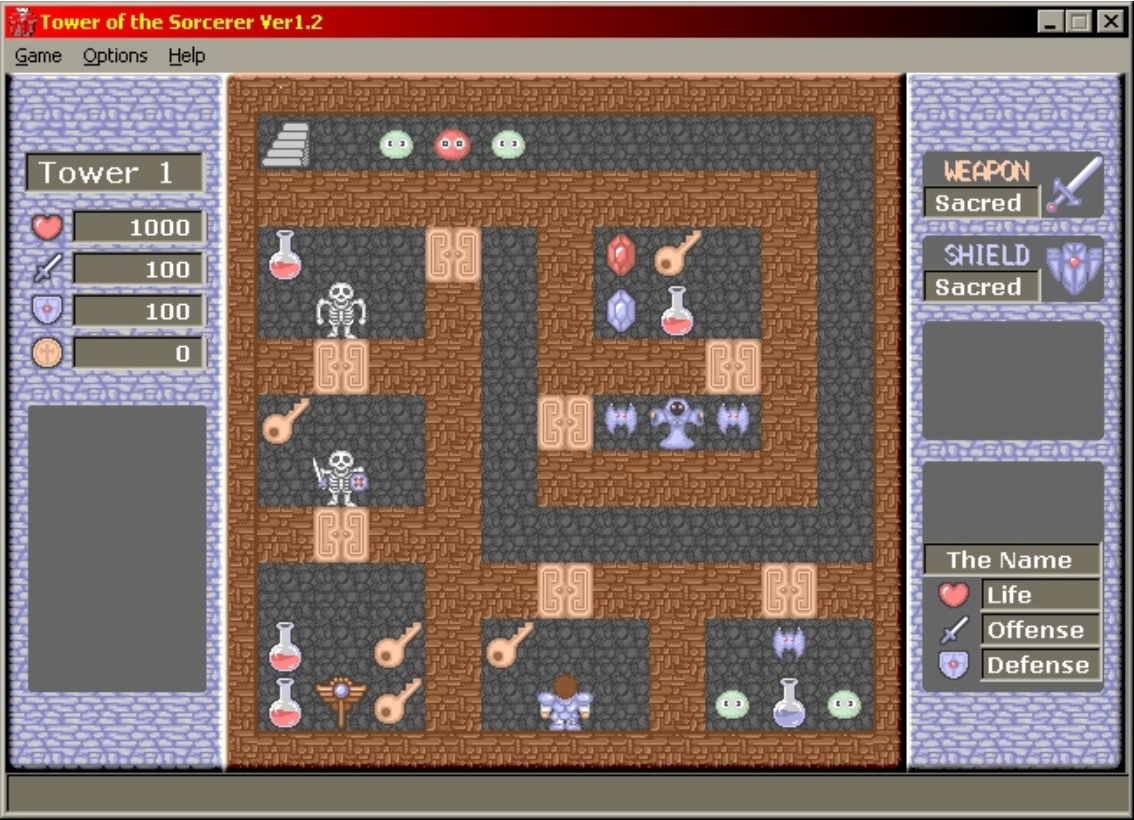
\includegraphics[width=0.8\textwidth]{src/tower.png}
    \caption{A Screenshot of the Gameplay.}
    \label{fig:gameplay}
\end{figure}


\section{Block Diagram}
In \reffig{fig:block_diagram}, the block diagram of the project is shown. There are a few main components in this block diagram:
\begin{itemize}
    \item The \textbf{User} controls the main character and the game UI via the USB keyboard.
    \item The \textbf{USB keyboard} interfaces with the NIOS II CPU.
    \item The \textbf{NIOS II CPU} interacts with the \textbf{On-chip memory} where the texture files are stored via the \textbf{Avalon Bus}. We will use tiles to store the visual design of the game elements.
    \item The \textbf{VGA controller} is responsible for displaying the current game state to the user so the user can decide next action to take.
    \item The \textbf{Game Logic Software} in the middle controls the gameplay and the interaction logic. 
\end{itemize}

\begin{figure}[h]
    \centering
    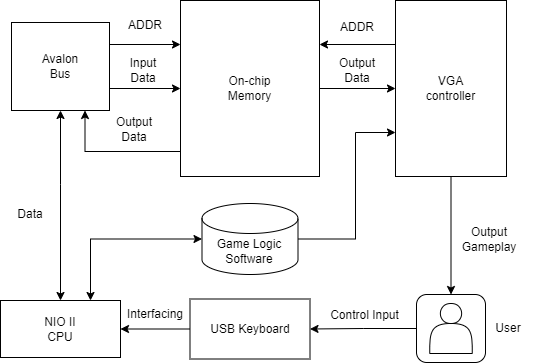
\includegraphics[width=0.8\textwidth]{block_diagram.png}
    \caption{The Block Diagram of the Implementation}
    \label{fig:block_diagram}
\end{figure}

\section{List of Features}
Given the complexity of the game logic, we aim to implement a subset of the following expected features:
\begin{itemize}
    \item Drawing the map with colored walls, floors, stairs, monsters, items, and the main character.
    \item The main character should interact with the environment correctly. \Eg, no glitches when walking, stoping at the wall, entering next floor when on the stairs blocks.
    \item The main character should be able to pick up and use items (\eg, keys, lotions), the effect should be reflected on the display immediately (\eg, keys opening doors, lostions increasing health bar)
    \item The main character should be able to combat with the monsters and the results should be intuitive (\eg, the health bar descreasing, monsters vanishing with an increase in gold)
    \item The main character should be able to interact with the NPC (Non-player characters) by dialoging and trading items.
    \item There should be some mandatory plots where the user is watching a fixed sequence of actions.
\end{itemize}

\section{Expected Difficulty}
The Difficulty mainly comes from the following aspects:
\begin{itemize}
    \item \textbf{Game Logic Implementation}. Being an RPG game, \textit{Tower of the Sorcerer} has multiple systems (\eg, the combat system, the character attribute system, the environment interaction system). We need to figure out the best way to make these systems interacting with each other properly.
    \item \textbf{Visual Design and Manipulation}. The game has rich visual elements. Statically, each of the numerous game elements (\eg, the main character, the monsters, the items, and environments such as floors, walls, doors) has multiple colors. We need to find a way to correctly store and fetch the needed color, without violating the memory constraints. Dynamically, when the player is interacting with the environment (\eg, switching back and forth the tower floors), the data for different floors should be displayed on the screen properly. The map state also needs to be tracked, (\eg, when the player goes from the second floor to the first floor, only the items left in the first floor should be displayed, not a completely new first floor).
    \item \textbf{Synchronization and Hardware Design}. The state of the character and the state of the game (\eg environment condition, item usage, monster attributes, character attributes) should be changed in a synchronous manner, \ie nothing should be lagging others. And this can be a potential issue when hardware delays and wait cycles are involved.
\end{itemize}

\section{Proposed Timeline}
For the four-week final project period, we plan to utilize the first week collecting game elements and building the minimal hardware implemnetation. During the second week, we aim to build a Minimal Viable Product with basic working functionalities of the game. The third and fourth weeks will be spent on implementing more features and debugging.


\end{document}
